	\documentclass[10pt,oneside]{CBFT_book}
	% Algunos paquetes
	\usepackage{amssymb}
	\usepackage{amsmath}
	\usepackage{graphicx}
% 	\usepackage{libertine}
% 	\usepackage[bold-style=TeX]{unicode-math}
	\usepackage{lipsum}

	\usepackage{natbib}
	\setcitestyle{square}

	\usepackage{polyglossia}
	\setdefaultlanguage{spanish}


	\usepackage{CBFT.estilo} % Cargo la hoja de estilo

	% Tipografías
	% \setromanfont[Mapping=tex-text]{Linux Libertine O}
	% \setsansfont[Mapping=tex-text]{DejaVu Sans}
	% \setmonofont[Mapping=tex-text]{DejaVu Sans Mono}

	%===================================================================
	%	DOCUMENTO PROPIAMENTE DICHO
	%===================================================================

\begin{document}

% =================================================================================================
\chapter{Ondas planas}
% =================================================================================================

Lejos de las fuentes de campo las ecuaciones de Maxwell son
\begin{align*}
	\divem{E} = 0 \qquad \qquad &\rotorm{E} = -\frac{1}{c}\dpar{\vb{B}}{t} \\
	\divem{B} = 0 \qquad \qquad &\rotorm{B} = \frac{1}{c}\dpar{\vb{E}}{t}
\end{align*}

Podemos derivar con respecto al tiempo en cada ecuación de rotor y reemplazar con la otra
de manera que
\[
	\rotorm{(\rotorm{B})} = \frac{1}{c}\dpar{}{t}\left(-\frac{1}{c}\dpar{\vb{B}}{t} \right)
	= \Nabla(\divem{B}) - \nabla^2 \vb{B}
\]
\[
	\rotorm{(\rotorm{E})} = -\frac{1}{c}\dpar{}{t}\left(\frac{1}{c}\dpar{\vb{E}}{t} \right)
	= \Nabla(\divem{E}) - \nabla^2 \vb{E}
\]
y esto nos lleva a 
\[
	\nabla^2 \vb{B} - \frac{1}{c^2}\dpar[2]{\vb{B}}{t} = 0 \qquad 
	\nabla^2 \vb{E} - \frac{1}{c^2}\dpar[2]{\vb{E}}{t} = 0
\]
dos sendas ecuaciones de onda para \vb{E} y \vb{B}. Pero es sabido que la solución de
\[
	\nabla^2 \psi - \frac{1}{c^2} \dpar[2]{\psi}{t} = 0
\]
es
\[
	\psi = A\euler^{i(\pe{k}{x}-\omega t)} + B\euler^{i(\pe{k}{x}-\omega t)}
\]
de modo que podemos postular como soluciones para nuestras ecuaciones de onda a
\[
	\vb{E} = \vec{\mathbb{E}}_0 \euler^{i(\pe{k}{x}-\omega t)} \qquad 
	\vb{B} = \vec{\mathbb{B}}_0 \euler^{i(\pe{k}{x}-\omega t)}
\]

Se tiene además que $\vb{k} = k \hat{n}$ da a través de $\hat{n}$ la dirección de
propagación de la onda. El número de onda $k$ podrá ser complejo lo cual refleja
atenuación. Las características del medio entran a través de
\[
	k = \sqrt{\mu\epsilon} \frac{\omega}{c}
\]
\notamargen{Acá hay que hacer las cuentas para demostrar todo esto que acá se
dice sin más. Además hay que comentar sobre la introducción de números complejos en
las amplitudes. Cómo son estos vectores complejos.}
Por su parte $\vec{\mathbb{E}}_0$ y $\vec{\mathbb{B}}_0$ son las amplitudes de los campos,
que serán números complejos constantes (no varían con la posición o el tiempo) y podrán
dar desfasajes.

Al utilizar las ecuaciones de divergencia sobre las soluciones se obtiene que 
\[
	\hat{n}\cdot \vec{\mathbb{E}}_0 = 0 \qquad \hat{n}\cdot \vec{\mathbb{B}}_0 = 0
\]
de manera que las ondas se propagan perpendicularmente a los campos, por ello las
ondas electromagnéticas son transversales.

Utilizando las ecuaciones de rotor de \vb{E}, en indicial (hacerlas), se llega a la importante 
relación 
\[
	\vec{\mathbb{B}}_0 = \sqrt{\mu\epsilon} \hat{n} \times \vec{\mathbb{E}}_0
\]
de modo que los vectores $\vec{\mathbb{E}}_0$ y $\vec{\mathbb{B}}_0$ también son perpendiculares.
Procediendo en forma análoga para la ley de Ampere-Maxwell se obtiene el mismo resultado.
Si el vector $\vb{k} \in \mathbb{R}$ entonces $\vec{\mathbb{E}}_0$ y $\vec{\mathbb{B}}_0$
tienen la misma fase.

En el vacío o en un medio LIH los campos \vb{E} y \vb{B} estarán en fase.
Asimismo $\vb{E}, \vb{B}, \hat{n}$ forman una terna derecha, lo cual se debe a que se definió
en primer lugar a $\vb{B}$ con una terna derecha. 

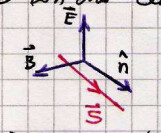
\includegraphics[width=0.2\textwidth]{images/fig_ft1_ondas_pic.jpg}

Luego,
\[
	\vb{S} \parallel \hat{n}
\]
si el medio es LIH pues $\vb{S} \propto \pv{E}{H} $. El vector de Poynting apunta en la
dirección de propagación de la onda.

En un medio anisótropo $\divem{D}=\divem{}(\epsilon \vb{E}) = 0$ siendo $\epsilon$ un tensor.
Allí $\vec{\mathbb{E}}_0 \cdot \hat{n} \neq 0$ salvo que $\epsilon$ esté diagonalizado y
$\vb{E} \parallel$ al eje principal.

Entonces si bien todavía se tiene que
\[
	\vb{S} = \frac{c}{4\pi} \left( \pv{E}{H} \right)
\]
pero si  $\vec{\mathbb{E}} $ ya no es perpendicular a $\hat{n}$ no será el vector de Poynting
$\vb{S}$ (dirección de propagación de la energía) paralelo a la dirección $\hat{n}$ de propagación 
de la onda.


\subsection{Sobre complejos}

El formalismo complejo es útil para operaciones lineales; cuando haya mangitudes no relacionadas
linealmente es un problema.
\[
	\mathcal{R}(A) = \frac{1}{2}( A + A^* )	\qquad \text{con} \; A \in \mathbb{C}
\]
Sean 
\[
	\vb{A}(\vb{x},t) = \vb{A}(\vb{x})\euler^{-i\omega t} \qquad \qquad 
			\vb{B}(\vb{x},t) = \vb{B}(\vb{x})\euler^{-i\omega t}
\]
siempre trabajaremos en general con dependencias temporales armónicas y metemos $\euler^{i\pe{k}{x}}$
en el módulo $\vb{A}_0$ que pasa a depender de $\vb{x}$.

Los campos físicos son siempre la parte real de las expresiones complejas.
Así, los campos físicos serán
\[
	\vb{A}(\vb{x},t) = \frac{1}{2} \left[ \vb{A}(\vb{x})\euler^{-i\omega t} + 
	\vb{A}^*(\vb{x})\euler^{i\omega t} \right]
\]
\[
	\vb{B}(\vb{x},t) = \frac{1}{2} \left[ \vb{B}(\vb{x})\euler^{-i\omega t} + 
	\vb{B}^*(\vb{x})\euler^{i\omega t} \right]
\]
La parte real de la suma es la suma de las partes reales,
\[
	\mathcal{R}(\vb{A} + \vb{B}) = \mathcal{R}( \vb{A} ) + \mathcal{R}( \vb{B} ),
\]
de modo que con operaciones lineales es lo mismo tomar parte real antes o después.
Pero para el producto,
\[
	\mathcal{R}(\vb{A}.\vb{B}) \neq  \mathfrak{R}( \vb{A} ) + \mathcal{R}( \vb{B} ),
\]
de modo que con operaciones no lineales no es lo mismo.
Para hacer producto necesito tomar la parte real de cada factor y entonces
\[
	\mathfrak{R}( \vb{A} ).\mathfrak{R}( \vb{B} ) = 
	\frac{1}{2}\mathfrak{R}( \vb{A}.\vb{B}^* + 
	\vb{A}.\vb{B} \euler^{ -i 2 \omega t }) =
	\frac{1}{2}\mathfrak{R}( \vb{A}^*.\vb{B} + 
	\vb{A}^*.\vb{B}^* \euler^{ i 2 \omega t }),
\]
donde el tercer término es porque a los efectos de tomar la parte real conjugar y no conjugar es lo
mismo.
Si $\vb{A}, \vb{B}$ son tales que tienen la misma fase, el resultado será real.

En las aplicaciones uno estará interesado en promedios temporales. El término con 
$\euler^{ i 2 \omega t}$ se hace nulo cuando el promedio es sobre un número entero de períodos,
entonces
\[
	\langle \vb{A} \vb{B} \rangle =
	\langle \mathfrak{R}( \vb{A} ).\mathfrak{R}( \vb{B} ) \rangle =
	\frac{1}{2} \: \mathfrak{R} ( \vb{A}.\vb{B}^* )
\]

\subsection{Poynting promedio y energías promedio}

Los campos \vb{E} y \vb{H} en ondas electromagnéticas toman la forma 
\[
	\vb{E} = \vec{\mathbb{E}}(\vb{x})\euler^{-i\omega t} \qquad 
	\vb{H} = \vec{\mathbb{H}}(\vb{x})\euler^{-i\omega t}
\]
de manera que 
\[
	\vb{S}( \vb{x},t ) = \frac{c}{4\pi} \frac{1}{2} \re( \vec{\mathbb{E}} \times \vec{\mathbb{H}}^* + 
		\vec{\mathbb{E}} \times \vec{\mathbb{H}} \euler^{-i2\omega t})
\]
\[
	\langle \vb{S}( \vb{x},t ) \rangle = \frac{c}{8\pi} \re( \vec{\mathbb{E}} \times \vec{\mathbb{H}}^* ) 
\]

En un MLIH es 
\[
	\vec{\mathbb{B}} = \sqrt{ \mu \epsilon } \hat{n} \times \vec{\mathbb{E}} \qquad\qquad 
	\vec{\mathbb{H}} = \sqrt{ \frac{\epsilon}{\mu } } \hat{n} \times \vec{\mathbb{E}}
\]
donde usamos que $\vb{H} = \vb{B}/\mu$, lo cual conduce a
\[
	\langle \vb{S}( \vb{x},t ) \rangle = \frac{c}{8\pi} \re( \vec{\mathbb{E}} \times 
		\sqrt{\frac{\epsilon}{\mu}}(\hat{n} \times \vec{\mathbb{E}})^* )
\]
\[
	\langle \vb{S}( \vb{x},t ) \rangle = \frac{c}{8\pi} \sqrt{\frac{\epsilon}{\mu}} 
		( \hat{n} (\vec{\mathbb{E}}\cdot\vec{\mathbb{E}}^*) - 
		\vec{\mathbb{E}}^*(\vec{\mathbb{E}}\cdot\hat{n}) )
\]
y finalmente
\[
	\langle \vb{S}( \vb{x},t ) \rangle = \frac{c}{8\pi} 
		\sqrt{\frac{\epsilon}{\mu}}|\vec{\mathbb{E}}|^2 \hat{n}
\]
que es el vector de Poynting para ondas en MLIH.
Se puede proceder en forma análoga para la energía. Entonces,
\[
	U(\vb{x},t) = \frac{1}{8\pi}( \pe{H}{B} + \pe{E}{D} )
\]
\[
	\langle U(\vb{x},t) \rangle = \frac{1}{8\pi} \frac{1}{2} \re ( 
	\vec{\mathbb{H}}\cdot\vec{\mathbb{B}}^* + \vec{\mathbb{E}}\cdot\vec{\mathbb{D}}^* )
\]
\[
	\langle U(\vb{x},t) \rangle = \frac{1}{16\pi}
		\re ( \frac{1}{\mu} |\vec{\mathbb{B}}|^2 + \epsilon |\vec{\mathbb{E}}|^2 ) =
		\frac{1}{8\pi} |\vec{\mathbb{E}}|^2
\]
puesto que 
\[
	|\vec{\mathbb{B}}|^2 = \mu\epsilon |\vec{\mathbb{E}}|^2,	
\]
y entonces la densidad de energía promedio es
\[
		\langle U(\vb{x},t) \rangle = \frac{1}{8\pi} |\vec{\mathbb{E}}|^2.
\]

% =================================================================================================
\section{Polarización de ondas}
% =================================================================================================

Una onda plana bien general en $\hat{n}$ es 
\be
	\vb{E}( \vb{x},t )=(\hat{\epsilon}_1 \vec{\mathbb{E}}_1 + 
			\hat{\epsilon}_2\vec{\mathbb{E}}_2) \euler^{i( \pe{k}{x} -\omega t)}
	\label{plane_wave_1}
\ee
Las amplitudes $\vec{\mathbb{E}}_1,\vec{\mathbb{E}}_2$ son complejos para permitir la diferencia 
de fase entre componentes.

\begin{figure}[htb]
	\begin{center}
	\includegraphics[width=0.4\textwidth]{images/fig_ft1_polariz.pdf} 
	\end{center}
	\caption{}
\end{figure} 

Si $\vec{\mathbb{E}}_1,\vec{\mathbb{E}}_2$ están en fase entonces $\vb{E}( \vb{x},t )$ está linealmente
polaridaza con $\theta$ fijo. Es como que \vb{E} viaja siempre por el mismo andarivel, oscilando. 

\begin{ejemplo}{\bf Polarización lineal}

Consideremos una onda que se propaga en $\zver$

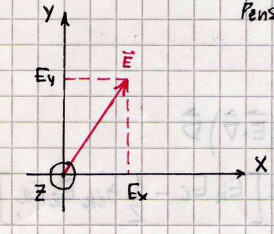
\includegraphics[width=0.25\textwidth]{images/fig_ft1_ondas_polarizacion_lineal.jpg} 

\[
	E_x = E_{0x} \cos( \omega t + \delta ) \qquad \qquad 
	E_y = E_{0y} \cos( \omega t )
\]
que son los valores que determinan la punta del vector en el tiempo.
Entonces
\[
	\frac{x^2}{E^2_{0x}} + \frac{y^2}{E^2_{0y}} - \frac{xy}{E_{0x}E_{0y}} \cos\delta = \sin^2\delta
\]
Si las dos componentes están en fase, $\delta = 0$ y de la ecuación anterior se deduce
\[
	y = \frac{ E_{0y} }{ E_{0x} } x.
\]
Onda linealmente polarizada.
\end{ejemplo}


Si $\vec{\mathbb{E}}_1,\vec{\mathbb{E}}_2$ tienen fase arbitraria entonces $\vb{E}( \vb{x},t )$ está elípticamente 
polarizada.

\begin{ejemplo}{\bf Polarización elíptica}

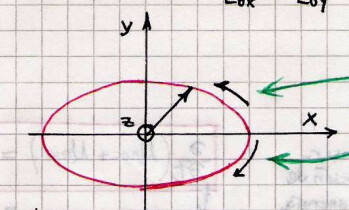
\includegraphics[width=0.25\textwidth]{images/fig_ft1_ondas_polarizacion_eliptica.jpg} 

Si $\delta = \pi/2$ entonces la ecuación resulta 
\[
	\frac{x^2}{E^2_{0x}} + \frac{y^2}{E^2_{0y}} = 1
\]
la punta del vector está sobre una elipse.
Puede ser sentido horario o antihorario.
Esto degenerará en una polarización circular; horaria (que lleva $\vb{L}$ en la dirección de $-\hat{k}$)
o antihoraria (que lleva $\vb{L}$ en la dirección de $\hat{k}$). Aquí la dirección $\hat{k}$ de la onda
es $\zver$.

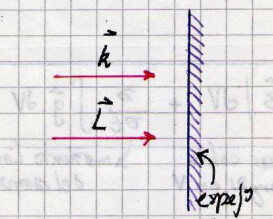
\includegraphics[width=0.25\textwidth]{images/fig_ft1_ondas_polarizacion_espejo.jpg} 

Pasará lo mismo con el momento angular $\vb{L}$ si incide una onda polarizada circularmente.
Aquí la superficie azul es un espejo. Incide una onda plana que le transfiere impulso lineal: hay presión
de radiación.

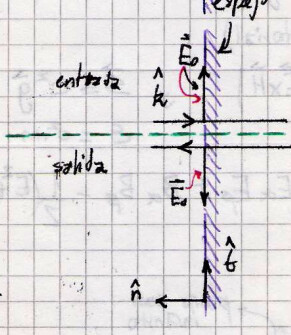
\includegraphics[width=0.25\textwidth]{images/fig_ft1_ondas_polarizacion_espejo2.jpg} 

Supongamos que al llegar al espejo (rebote) el campo $\vb{E}$ sea en la dirección $\hat{t}$.
Como $ \hat{n} \times (\vb{E}_1 - \vb{E}_2 ) = 0$ se desfase $\pi$.
Los contornos en los casos dinámicos son iguales a los estáticos.

Estamos reflejando la onda y no se altera el \vb{L} porque relfejanos el sistema y al ser \vb{L} vector axial
no debe sufrir cambios.
\notamargen{Como está circularmente polarizada, la onda lleva momento angular \vb{L}.} 
 
\end{ejemplo}

Si $|\vec{\mathbb{E}}_1|=|\vec{\mathbb{E}}_2|$ y la fase es $\pi/2$ entonces $\vb{E}( \vb{x},t )$ está circularmente 
polarizada.

\[
	\vec{\mathbb{E}}_2 = \vec{\mathbb{E}}_1 \euler^{i \pi/2} =\vec{\mathbb{E}}_1 i
\]
entonces
\[
	\vb{E}( \vb{x},t )= \vec{\mathbb{E}}_1 (\hat{\epsilon}_1  \pm \hat{\epsilon}_2 )
				\euler^{i( \pe{k}{x} -\omega t)}	
\]
\notamargen{Revisar porque en la carpeta no coincide. Se tiene en cambio lo que pongo en el ejemplo
par dinamitar.}
\begin{ejemplo}{\bf Para dinamitar}
\[
 	\vb{E}( \vb{x},t )= \vec{\mathbb{E}}_1 (\hat{\epsilon}_1 \pm i \: \hat{\epsilon}_2 )
				\euler^{i( \pe{k}{x} -\omega t)}
\]
donde el $+$ es horario y el $-$ antihorario (momento angular en el sentido de propagación).
\end{ejemplo}
donde el $+$ corresponde a $\mathcal{C}^+$ antihoraria y el $-$ a horaria. Nos definimos por comodidad,
\[
	\hat{\epsilon}_+ \equiv \frac{\hat{\epsilon}_1 + i \hat{\epsilon}_2 }{\sqrt{2}} \qquad\qquad 
	\hat{\epsilon}_- = \frac{\hat{\epsilon}_1 - i \hat{\epsilon}_2 }{\sqrt{2}}
\]
una base de polarizaciones. Se cumplen
\[
	\hat{\epsilon}_\pm \cdot \hat{\epsilon}_\mp^* = 0 \qquad \qquad 
	\hat{\epsilon}_\pm \cdot \hat{\epsilon}_\pm^* = 1
\]
\[
	\hat{\epsilon}_1 = \sqrt{2}( \hat{\epsilon}_+ + i \hat{\epsilon}_- ) \qquad \qquad 
	\hat{\epsilon}_2 = \sqrt{2}( \hat{\epsilon}_+ - i \hat{\epsilon}_- )
\]
luego cualquier polarización se puede escribir como combinación lineal de $\mathcal{C}^+$ y $\mathcal{C}^-$.

Por otra parte, una onda plana general también se puede escribir, además de como en
\eqref{plane_wave_1}, según
\[
	\vb{E}( \vb{x},t )=(\hat{\epsilon}_+ \vec{\mathbb{E}}_+ + 
			\hat{\epsilon}_-\vec{\mathbb{E}}_-) \euler^{i( \pe{k}{x} -\omega t)}
\]
donde la conversión entre bases la tenemos en las expresiones previas. Luego,
\[
	\frac{E_1}{E_2} = \frac{1 + E_-/E_+}{1 - E_-/E_+} =\frac{|1+r|}{|1-r|} \qquad \qquad 
	\frac{E_-}{E_+} = r \euler^{i\alpha}
\]
Entonces
\[
	\vb{E} = \Frac{E_+ + E_-}{\sqrt{2}} \hat{\epsilon}_1 + 
	i \Frac{ E_+ - E_- }{\sqrt{2}}\hat{\epsilon}_2
\]
donde el cambio de bases es
\[
	\begin{pmatrix}
	\hat{\epsilon}_+ \\
	\\
	\hat{\epsilon}_-
	\end{pmatrix} =
	\begin{pmatrix}
	\frac{1}{\sqrt{2}} & \frac{i}{\sqrt{2}} \\
	\\
	\frac{1}{\sqrt{2}} & \frac{-i}{\sqrt{2}}
	\end{pmatrix}
	\begin{pmatrix}
	\hat{\epsilon}_1 \\
	\\
	\hat{\epsilon}_2
	\end{pmatrix} =
	T_1 
	\begin{pmatrix}
	\hat{\epsilon}_1 \\
	\\
	\hat{\epsilon}_2
	\end{pmatrix}
\]
\[
	\begin{pmatrix}
	\hat{\epsilon}_1 \\
	\\
	\hat{\epsilon}_2
	\end{pmatrix} =
	\begin{pmatrix}
	\frac{1}{\sqrt{2}} & \frac{1}{\sqrt{2}} \\
	\\
	\frac{-i}{\sqrt{2}} & \frac{i}{\sqrt{2}}
	\end{pmatrix}
	\begin{pmatrix}
	\hat{\epsilon}_+ \\
	\\
	\hat{\epsilon}_-
	\end{pmatrix} =
	T_1^{-1} 
	\begin{pmatrix}
	\hat{\epsilon}_+ \\
	\\
	\hat{\epsilon}_-
	\end{pmatrix}
\]
donde $T_1, T_2$ son transformaciones que nos llevan de una base a otra por
rotación de los versores.
\[
	T_2 = 	\begin{pmatrix}
	\cos x & \sin x \\
	\\
	- \sin x & \cos x 
	\end{pmatrix}
\]
\[
	\begin{pmatrix}
	\hat{\epsilon}_1' \\
	\\
	\hat{\epsilon}_2'
	\end{pmatrix} =
	T_2
	\begin{pmatrix}
	\hat{\epsilon}_1 \\
	\\
	\hat{\epsilon}_2
	\end{pmatrix}
\]
\[
	\begin{pmatrix}
	\hat{\epsilon}_+' \\
	\\
	\hat{\epsilon}_-'
	\end{pmatrix} =
	T_1 T_2
	\begin{pmatrix}
	\hat{\epsilon}_1 \\
	\\
	\hat{\epsilon}_2
	\end{pmatrix}
\]
con
\[
	T_1 T_2 = \begin{pmatrix}
	\euler^{-ix} & 0 \\
	\\
	0 & \euler^{ix}
	\end{pmatrix}
\]

Ahora se cambia de base la onda \vb{E}, lo cual da
\[
	\vb{E} = \left[ \euler^{ix} E_+ \hat{\epsilon}_+ + \euler^{-ix} E_- \hat{\epsilon}_- \right]
	\euler^{i \pe{k}{x} - i \omega t}
\]
y pasamos a una nueva base donde la elipse es canónica.
\[
	\frac{E_-'}{E_+'} = \frac{E_-}{E_+} \euler^{-2 i x} = r \euler^{ i \alpha} \euler^{-2 i x}
\]
Habiendo girado $\alpha/2$ hemos hecho coincidir con los ejes los semiejes principales
de la elipse.

Una onda que rebota en un espejo transfiere impulso lineal. Una onda $\mathcal{C}$ lleva \vb{L} pero no lo transfiere 
en un rebote perfecto. Por ser \vb{L} un vectorial axial (pseudovector) el reflejo es equivalente a una simetría del 
sistema.

Tenemos dos base entonces $\{ \hat{\epsilon}_1 ,\hat{\epsilon}_2 \}$ y $\{ \hat{\epsilon}_+ ,\hat{\epsilon}_- \}$.
Además,
\[
	\frac{\vec{\mathbb{E}}_-}{\vec{\mathbb{E}}_+} = r\euler^{i\alpha} 
\]
si $r = \pm 1, \alpha=0 $ entonces estamos frente a linealmente polarizada.

\subsection{El tensor de Maxwell para las ondas}

Para la onda plana hay direcciones privilegiadas. Fijemos
\[
	x : \text{ campo } \vb{E} \qquad 
	y : \text{ campo } \vb{B} \qquad 
	z : \text{ propagación }
\]
El tensor será
\[
	T = \frac{1}{4\pi} \: \begin{pmatrix}
	        0	& 0 	& 0 \\
		0	& 0	& 0 \\
		0	& 0	& -2\epsilon|\vb{E}_0|^2
	       \end{pmatrix}
\]
donde los ceros en los dos elementos diagonales superiores se deben a que no transmite impulso en una
dirección que no es la de propagación. 
Luego, el valor promedio temporal será
\[
	\langle T \rangle =  \langle T_E \rangle + \langle T_M \rangle
\]
que lleva a
\[
	- \epsilon|\vb{E}_0|^2  - \frac{1}{\mu} |\vb{B}_0|^2 = -2\epsilon|\vb{E}_0|^2
\]

En el ejemplito que ilustra esta figura [Chequear esto que es super sketchi!]

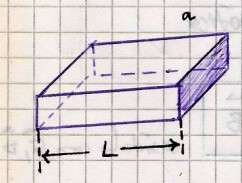
\includegraphics[width=0.225\textwidth]{images/fig_ft1_paraTensorOndasMax.jpg}
	
\[
	E = \langle \mu \rangle a L = \langle \vb{S} \rangle a t
\]
puesto que $t=L/v$ y donde $v = \langle S \rangle / \langle \mu \rangle  = c / \sqrt{\mu \epsilon}$.
Se ve que 
\[
	\langle \vb{S} \rangle =  \frac{c}{8\pi} \sqrt{ \frac{\varepsilon}{\mu} }|\vb{\epsilon}|^2
	\langle \mu \rangle = \frac{\varepsilon}{8\pi}  |\vb{\epsilon}|^2
\]

% =================================================================================================
\section{Reflexión y refracción de ondas en medios}
% =================================================================================================

Consideramos una onda plana que llega a una separación entre medios transparentes.
Las condiciones de contorno deben adaptarse a la dinámica, pero las ecuaciones de las divergencias
\[
	\divem{B} = 0 \qquad \divem{D} = 0
\]
se mantienen iguales al caso estático de manera que no variará el contorno que dependa de ellas.
No olvidemos que las fuentes están muy lejos y entonces $\rho \sim 0$ y $\vb{J} \sim 0$.

Los medios son LIH y transparentes. Las ecuaciones de rotor serán
\[
	\rotorm{E} = -\frac{1}{c} \dpar{\vb{B}}{t} \qquad 
	\rotorm{H} = \frac{1}{c} \dpar{\vb{D}}{t}
\]
Luego las condiciones de contorno son las mismas que para el caso estático.

Partimos de una onda
\[
	\vb{E}( \vb{x},t )= \vec{\mathbb{E}}_0 \euler^{i( \pe{k}{x} -\omega t)}
\]
donde 
\[
	k = \sqrt{\mu\epsilon} \frac{\omega}{c} = \frac{\omega}{v}
\]
siendo $v$ la velocidad en el medio. Los índices de refracción serán 
\[
	n = \sqrt{\mu \epsilon} \qquad  n' = \sqrt{\mu' \epsilon'}
\]
de tal suerte que los campos son 
\[
	\vb{B} = \frac{\sqrt{\mu\epsilon}}{k} \; \pv{k}{E} \qquad \quad 
		\vb{H} = \sqrt{\frac{\epsilon}{\mu}} \frac{1}{k} \; \pv{k}{E}
\]
\begin{figure}[htb]
	\begin{center}
	\includegraphics[width=0.7\textwidth]{images/fig_ft1_reflex1.pdf}	 
	\end{center}
	\caption{}
\end{figure} 

Las ondas reflejada y transmitida serán, respectivamente,
\[
	\vb{E}'' = \vec{\mathbb{E}}_0'' \euler^{i( \pe{k''}{x} -\omega'' t)} \qquad 
	\vb{E}' = \vec{\mathbb{E}}_0' \euler^{i( \pe{k'}{x} -\omega' t)},
\]
pero como el medio $''$ y el sin primar es el mismo ($\mu''= \mu, \epsilon''=\epsilon$) 
se tendrá 
\[
	|\vb{k}| = |\vb{k}''|.
\]

Se quiere saber si al cruzar de un medio al otro cambia $\omega$, $k$ o ambas.
Notemos que las condiciones de contorno se deben satisfacer sobre el contorno durante
todo instante de tiempo, entonces las fases de las tres ondas
\[
	\pe{k}{x}\:|_{z=0} - \omega t = 
	\pe{k'}{x}\:|_{z=0} - \omega' t  = 
	\pe{k''}{x}\:|_{z=0} - \omega t 
\]
y $\omega' = \omega $ dado que ambas tienen que ser iguales término a término 
(parte espacial y parte temporal).
Entonces la frecuencia $\omega$ no varía entre medios, lo que varía es la longitud
de onda.

Esto conduce a
% \[
% 	\omega t = \omega' t = \omega'' t
% \]
\[
	\pe{k}{x}\:|_{z=0} = \pe{k'}{x}\:|_{z=0}  = \pe{k''}{x}\:|_{z=0} 
\]
Pero notemos que $ \nver \cdot \vbx|_{z=0} = 0$ y que se puede escribir
\[
	\vb{x}|_{z=0} = \vbx (\nver\cdot\nver) - (\nver\cdot\vbx)\nver |_{z=0},
\]
y entonces
\[
	\vb{k}\cdot [ \nver \times ( \vbx \times \nver ) ]_{z=0} =
	\vb{k}'\cdot [ \nver \times ( \vbx \times \nver ) ]_{z=0} =
	\vb{k}''\cdot [ \nver \times ( \vbx \times \nver ) ]_{z=0}
\]
y esto es la ecuación de un vector contenido en un plano. Luego, los tres vectores 
$\vb{k}, \vb{k}', \vb{k}''$  tienen un plano en común.

Con esto se obtiene la primer ley de la óptica geométrica, habiendo postulado la mera
existencia de condiciones de contorno. Los vectores que representan las ondas están
en un mismo plano y se verifica
\[
	k \sin(i) = k' \sin(r) = k'' \sin(i'),
\]
y se deducen las consecuencias
\[
	n \sin (i) = n' \sin(i') \qquad \text{Ley de Snell},
\]
donde $n = \sqrt{\mu \epsilon}$ y que el ángulo de incidencia es igual al de reflexió
\[
	i = i' \qquad \text{Ley de reflexión}.
\]

La existencia de condiciones de contorno en $z=0$ que deben ser satisfechas en todo $t$ 
en todo punto $(x,y)$ lleva a todos los factores de fase iguales en $z=0$. 

Se debe tener \vb{B} normal continuo y \vb{D} normal continuo también, lo 
cual viene de $\divem{B}=0$ y $\divem{D}=0$.

% La frecuencia $\omega$ es la misma para el medio 1 y el medio 2 pues $\lambda_1 \neq \lambda_2$.
% Los tres vectores $\vb{k}, \vb{k}', \vb{k}''$ están en un mismo plano, entonces 

Luego se plantean los contornos considerando que los campos bajo $z=0$ son suma de
incidente y reflejado.
\[
	D_{\nver} : \qquad [ \vb{D}_2 - \vb{D}_1 ]\cdot\hat{n} = 0 \qquad \rightarrow  \qquad 
		[ \epsilon'\vb{E}_0^{'} - \epsilon (\vb{E}_0 + \vb{E}_0^{''} )  ]\cdot\hat{n} = 0
\]
\[
	E_{\hat{t}} : \qquad \hat{n} \times [ \vb{E}_2 - \vb{E}_1 ] = 0 \qquad \rightarrow \qquad 
		\hat{n} \times [ \vb{E}_0^{'} - (\vb{E}_0 + \vb{E}_0^{''} )  ]  = 0
\]
\[
	B_{\hat{n}} : \qquad  [ \vb{k}' \times \vb{E}_0^{'} - ( \vb{k} \times \vb{E}_0 + 
			\vb{k}'' \times \vb{E}_0^{''} )  ]\cdot\hat{n} 
\]
\notamargen{Igual a cero esto?}
\[
	H_{\hat{t}} : \qquad  \hat{n} \times \left[ \frac{1}{\mu'}\vb{k}' \times \vb{E}_0^{'} - 
			\frac{1}{\mu}( \vb{k} \times \vb{E}_0 + \vb{k}'' \times \vb{E}_0^{''} ) \right]  = 0
\]
de manera que 
\[
	\vb{B} = \frac{\sqrt{\mu\epsilon}}{k} \pv{k}{E} = \frac{c}{\omega} \pv{k}{E} \qquad \qquad 
	\vb{H} = \frac{c}{\mu \omega } \pv{k}{E}
\]
donde $c/\omega$ es el mismo para ambos medios.

Aplicando diligentemente los contornos se llega a las {\it relaciones de Fresnel} que son los cocientes de las 
amplitudes relativas.

\notamargen{Pese a que el rotor de \vb{E} es no nulo en dinámica, para los contornos
vale lo mismo que para el caso estático.}

Analicemos primeramente el transverso eléctrico, cuya situación está depicted en la figura

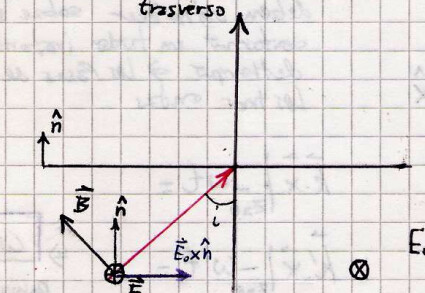
\includegraphics[width=0.4\textwidth]{images/fig_ft1_ondas_TE.jpg} 

La condición de $D_{\nver}$ se satisface idénticamente, y
\[
	- \vb{E}_0^{'} + \vb{E}_0 + \vb{E}_0^{''} = 0,
\]
luego, usando que $ (\pv{k}{E})\cdot\nver= (\vb{E}_0\times\nver)\cdot\vb{k} = E_0 \: k \sin(i)$
se tiene
\[
	(\pv{k}{E})\times\nver = -\vb{k} (\nver\cdot\vb{E}_0) + \vb{E}_0 (\nver\cdot\vb{k}) =
	E_0'\: k \: \cos( i )
\]
que conduce a
\[
	\sqrt{\frac{\epsilon}{\mu}} (E_0 - E_0'') \cos( i ) -
	\sqrt{\frac{\epsilon'}{\mu'}} E_0' \cos( r ) = 0.
\]
donde se ha usado también que
\[
	k'= k \sqrt{\frac{\mu'\epsilon'}{\mu\epsilon}}.
\]
Entonces
\[
	\frac{E_0^{''}}{E_0} = \frac{1 - \frac{\mu\tan(i)}{\mu'\tan(r)} }{ 1 + \frac{\mu\tan(i)}{\mu'\tan(r)} } 
	\approx -\frac{\sin(i-r)}{\sin(i+r)}
\]
donde la última aproximación es porque para medios transparentes se tiene $\mu \sim 1$.
Asimismo
\[
	\frac{E_0^{'}}{E_0} = \frac{ 2 }{1 + \frac{\mu}{\mu'} \frac{\tan(i)}{\tan(r)} } =
	1 + \frac{\sin(r-i)}{\sin(r+i)}
\]

Sea la situación $ r < i $ y $ n' < n $, entonces se tendrán:

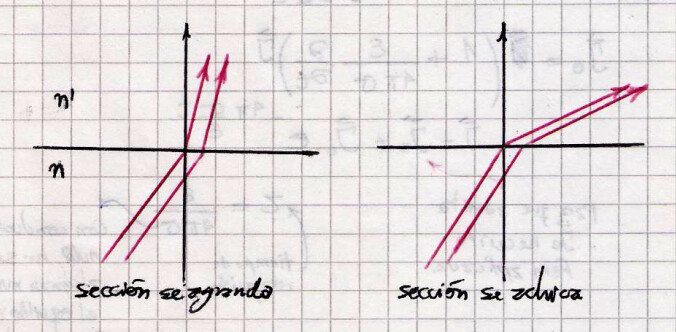
\includegraphics[width=0.5\textwidth]{images/fig_ft1_ondas_TE2.jpg} 

Analicemos ahora el transverso magnético
\notamargen{¿trans o tras?}

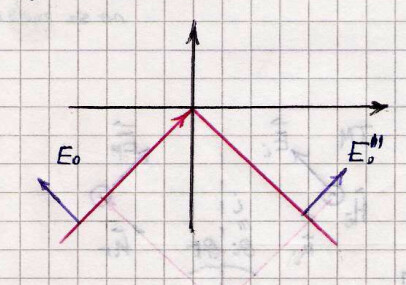
\includegraphics[width=0.5\textwidth]{images/fig_ft1_ondas_TM.jpg} 

Haciendo los cálculos se llega a
\[
	\frac{E_0^{''}}{E_0} = \frac{ -\frac{\mu}{\mu'} \sin(2r) + \sin(2i) }
	{ \frac{\mu'}{\mu} \sin(2r) + \sin(2i) } 
	\approx \frac{ \tan(i-r)}{\tan(i+r)}
\]
\[
	\frac{E_0^{'}}{E_0} = 2 \sqrt{ \frac{\mu\epsilon}{\mu'\epsilon'} }
	\frac{ \sin( 2i ) }{ \sin(2r) + \frac{\mu}{\mu'}\sin(2i) }
	\approx \frac{ 2 \sin(r) \cos( i) }{\sin(i+r) \cos(i-r) }
\]
donde las últimas igualdades en cada caso se obtienen usando medio transparente.

Usando $\mu \sim 1$ (válido para medios transparentes) tenemos

\[
	TE \qquad \qquad TM
\]
\[
	\frac{E_0^{''}}{E_0} = -\frac{\sin(i-r)}{\sin(i+r)} \qquad \qquad 
	\frac{E_0^{''}}{E_0} = \frac{\tan(i-r)}{\tan(i+r)} 
\]
\[
	\frac{E_0^{''}}{E_0} = 1 + \frac{\sin(r-i)}{\sin(i+r)} \qquad \qquad 
	\frac{E_0^{''}}{E_0} = \frac{2 \sin(r)\cos(i)}{\sin(i+r)\cos(i-r)} 
\]
\begin{figure}[htb]
	\begin{center}
	\includegraphics[width=0.7\textwidth]{images/fig_ft1_reflex2.pdf} 
	\end{center}
	\caption{}
\end{figure} 

\notamargen{frecuencias ópticas $\mu'/\mu = 1$}.

Si $i \sim 0$ entonces TE y TM son similares a menos de un signo, el cual es debido
solamente a la convención asumida para los campos a la entrada y a la salida.

Si $i+r = \pi/2$ el TM es nulo y el ángulo $i$ es el ángulo de Brewster.

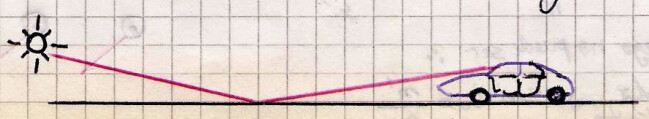
\includegraphics[width=0.5\textwidth]{images/fig_ft1_ondas_autete.jpg} 

Cuando case el sol será más molesta la luz reflejada pero se puede evitar con un
polarizador ubicado convenientemente.

Recordemos que el campo \vb{E} es el vector que caracteriza el vector óptico, lo cual
se ve en experiencias de Lloyd? o Wiener?.

Notemos que  
\[
	\vb{S}_i \neq \vb{S}_r + \vb{S}_t ,
\]
pues \vb{S} no está relacionado linealmente con \vb{E}, \vb{B}, y lo que sí vale es
\[
	\vb{S}_i \cdot \hat{n} = \vb{S}_r \cdot \hat{n} + \vb{S}_t \cdot \hat{n}.
\]

\subsubsection{Polarization (Brewster angle)}

Es un $i_B$ tal que no hay onda \vb{E} reflejada (en TM),
\[
	E_0^{''} = 0,
\]
pues $\tan( i + r) \to \infty$ con $i+r =\pi/2$ se da
\[
	i_b = \atan \left( \frac{n'}{n}\right) ,
\]
y entonces 
\[
	\frac{n}{n'}\sin(i_B) = \cos(i_B) \rightarrow i_b = \atan\left( \frac{n'}{n}\right),
\]
Sirve para producir luz polarizada linealmente.

\begin{figure}[htb]
	\begin{center}
	\includegraphics[width=0.4\textwidth]{images/fig_ft1_reflex3.pdf}	 
	\end{center}
	\caption{}
\end{figure} 

No puede suceder Brewster y reflexión total interna simultáneamente (¿se come la onda el medio?)

\subsubsection{Reflexión interna total}

Sea $ n_{inc} > n_{trans} $. Entonces se da que
\[
	n \sin(i) = n'\sin(r),
\]
\[
	\frac{n}{n'} \sin(i) = \sin(r),
\]
y el LHS es mayor igual a 1 para algunos $i$. Existe un ángulo límite 
\[
	\sin(r) = 1 = \frac{n}{n'} \sin(i) 
\]
\[
	i_0 = \asen\left( \frac{n'}{n} \right)
\]
de manera que si $i \geq i_0$ entonces $\sin(r) > 1$ y se debe tener un $r\in \mathbb{C}$.

\begin{figure}[htb]
	\begin{center}
	\includegraphics[width=0.4\textwidth]{images/fig_ft1_reflex4.pdf}	 
	\end{center}
	\caption{}
\end{figure} 

\notamargen{Tenía este sketch para la convención de TM y TE:
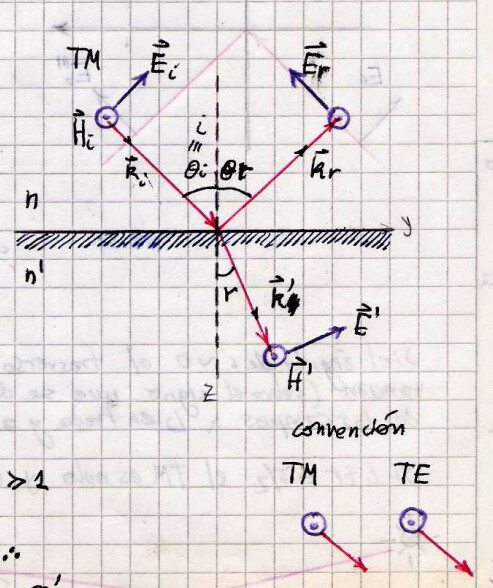
\includegraphics[width=0.32\textwidth]{images/fig_ft1_ondas_convencion.jpg}
}

Si $\sin(r)>1$ se tiene $\sin(r)^2 > 1$ y como por teorema de Pitágoras es 
\[
	\cos(r)^2 = 1 - \sin(r)^2 \rightarrow \cos(r) = i \sqrt{ \sin(r)^2 - 1 }
\]
donde notemos especialmente que hemos sacado fuera un $\sqrt{-1} = i$ para que el argumento 
de la raíz sea positivo en este caso especial. Luego 
\[
	\cos(r) = i \sqrt{ \frac{n}{n'}\sin(i)^2 - 1 } = i a 
\]
y si $\sin(r) = 1$ entonces $r = \pi/2$.
Entonces
\[
	\euler^{i(\vb{k}\cdot\vb{x})} = \euler^{i(k \cos(r)z + k \sin(r)x)} =
		\underbrace{\euler^{-kaz}}_{\text{atenuación}} 
		\underbrace{\euler^{ik\sin(r)x}}_{\text{propagación}}
\]
Hay ondas evanescentes en la reflexión interna total

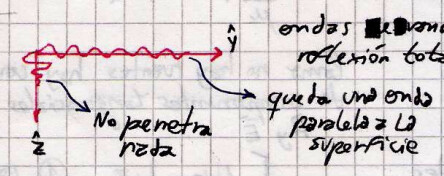
\includegraphics[width=0.4\textwidth]{images/fig_ft1_reflexion_total.jpg}

El vector de onda $\vb{k}'$ se puede pensar como un $\vb{k}'= k'\cos(r) - ik'\sin(r)$ aunque
este pensamiento no es muy feliz (anoté).


\begin{ejemplo}{\bf Problema 1}
 
Se trata de reflexión interna total.
Se considera el promedio de $\vb{S}$ porque alterna en el tiempo, luego
\[
	\vm{\vb{S}\cdot\nver} = \frac 1 2 \mathcal{Re}\left( \frac{c}{4\pi} 
	\vb{E}\times\vb{H}^*\right) \cdot \nver
\]
y entonces
\[
	\frac 1 2 \mathcal{Re}\left( S'\hat{k}'\cdot\nver \right) =
	\frac 1 2 \mathcal{Re}\left( \frac{c}{4\pi} 
	\vb{E}'\times\sqrt{\epsilon}( \hat{k}'\times\vb{E})^*\right)
\]

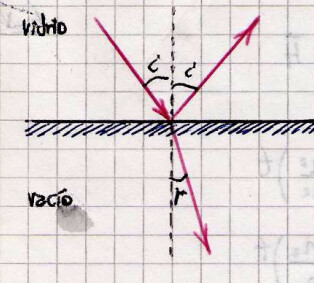
\includegraphics[width=0.3\textwidth]{images/fig_ft1_problema1_ondas.jpg}

\[
	\vm{\vb{S}\cdot\nver} = \frac{1}{2}  \mathcal{Re}\left( 
	\sqrt{\epsilon} \frac{c}{4\pi} |\vb{E}|^2 \hat{k}^*\cdot\nver \right)
\]
\[
	\vm{\vb{S}\cdot\nver} = \frac{1}{2} \frac{ \sqrt{\epsilon} c}{4\pi} |\vb{E}|^2
	\mathcal{Re}\left( \cos r \right)
	= 0,
\]
lo cual es nulo porque es imaginario puro el coseno, entonces no hay flujo del vector 
de Poynting hacia abajo.
 
\end{ejemplo}


\begin{ejemplo}{\bf Problema 3}

Se considera incidencia normal. En el dibujete están esquematizadas direcciones y medidas

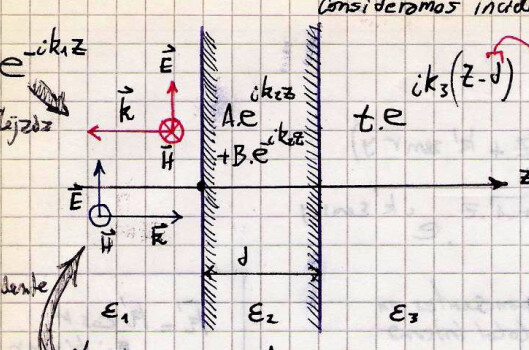
\includegraphics[width=0.4\textwidth]{images/fig_ft1_problema3A_ondas.jpg}

Se plantean dos coeficientes en el medio porque hay una onda que viene y una que va. En la incidencia
no escribimos explícitamente la parte temporal $i \omega t$ y el coeficiente se toma $E_0=1$.
Consideramos $\mu=1$ y se obtendrá $\vb{H}$ a partir de $\vb{E}$ según
\[
	\vb{H} = \frac{n}{\mu} \hat{k}\times\vb{E}
\]

Como no hay fuentes, hay continuidad de componentes tangenciales de $\vb{H}$ y $\vb{E}$,
\[
	z = 0 \qquad 	\begin{cases}
			\; 1 + r = A + B \qquad\qquad \textcircled{1} \text{ campo } \vb{E} \\
			\\
			\; n_1 ( 1 - r ) = n_2 ( A - B ) \qquad \qquad \textcircled{2} \text{ campo } \vb{H}
			\end{cases}
\]
\[
	z = d \qquad 	\begin{cases}
			\; A \euler^{i k_2 d} + B \euler^{-i k_2 d} = t 
			\qquad\qquad \textcircled{3} \text{ campo } \vb{E} \\
			\\
			\; n_3 ( A \euler^{i k_2 d} - B \euler^{-i k_2 d} ) = n_3 t 
			\qquad\qquad \textcircled{4} \text{ campo } \vb{H} \\
			\end{cases}
\]

Entonces, se despejan $A,B$ desde \textcircled{3} y \textcircled{4}, dando
\[
	A \euler^{ i k_2 d } = \frac 1 2 \left( 1 + \frac{ n_3 }{ n_2 } \right) t \qquad \qquad 
	B \euler^{ - i k_2 d } = \frac 1 2 \left( 1 - \frac{ n_3 }{ n_2 } \right) t
\]
y utilizando estas junto con \textcircled{1} y \textcircled{2}
\[
	\frac{1+r}{1-r} = \frac{n_1}{n_2} \Frac{ 1 + r_{23} \euler^{2ik_2d}}{ 1 - r_{23} \euler^{2ik_2d} }
	\qquad \qquad r_{23} \equiv \frac{1 - n_3/n_2}{1 + n_3/n_2}
\]
siendo este último $r_{23}$ el coeficiente de reflexión del medio 2 al 3.
Ahora buscaremos cuándo se anula esta cosa.
\[
	r = \frac{ r_{12} - r_{23} \euler^{i 2 k_2 d} }
	{ 1 + r_{12} r_{23} \euler^{i 2 k_2 d} }
	\qquad \qquad r_{12} \equiv \frac{n_2 - n_1}{n_2 + n_1}
\]
y la anulación de partes real e imaginaria requiere
\[
	r_{12} + r_{23} \euler^{i \delta} = 0 
\]
\[
	r_{12} + r_{23}\cos\delta = 0 \qquad r_{12} + r_{23}\sin\delta = 0
\]
luego, si $ \delta = 2 k_2 d = m \pi $ será
\[
	r_{12} + r_{23}(-1)^m = 0,
\]
y con $m$ par
\[
	r_{12} = -r_{23} \qquad r_{12} = -r_{21}
\]
se invierte el orden de los medios. Una solución razonable es $n_3=n_1$ que lleva a $r_{21} = r_{23}$.
Con $m$ impar se tienen $ r_{12} = r_{23} $ que lleva a $n_2^2 = n_3 n_1$.

{\bf Forma alternativa}

Esto se puede resolver de una forma alternativa, como en interferencia. Veamos el dibujete

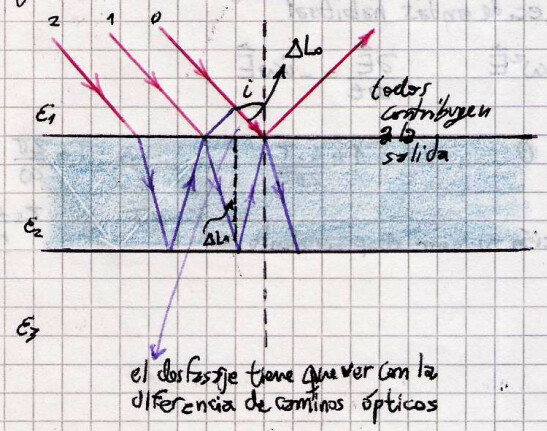
\includegraphics[width=0.4\textwidth]{images/fig_ft1_problema3B_ondas.jpg}
 
se tiene que
\[
	\vb{E} = \sum_{j=0}^\infty \: \vb{E}_j \euler^{i \delta_j }
\]
y será
\[
	\delta = \k_2 \Delta L_1 - k_1 \Delta L_0
\]
\[
	\Delta L_1 = 2 \Frac{d}{\cos r} \qquad \qquad 
	\Delta L_0 = 2 d \tan r \sin i
\]
y haciendo cálculos
\[
	\delta = \frac{2 d \omega }{c} n_2 \cos r
\]
con cada rayo se suma al desafasaje $\delta$.
\notamargen{Estamos haciendo $\delta_j = j \delta $.}

Para las amplitudes se tiene
\[
	E_0 = r_{12} E_i \qquad E_j = t_{21} r_{23}^j r_{21}^{j-1} t_{12} E_i,
\]
y los primeros se pueden hacer {\it a mano}, así
\[
	E = \left[ \: r_{12} + \frac{t_{12}t_{21}}{r_{21}} \sum_{j=1}^\infty \: 
	( r_{23} r_{21} \euler^{i\delta} )^j \: \right] E_i = 
	\left[ \: r_{12} + \frac{t_{12}t_{21}}{r_{21}} \: 
	\frac{ r_{23} r_{21} \euler^{i\delta} }{1 - r_{23} r_{21} \euler^{i\delta} } \: \right] E_i 
\]
y usando $ t_{12} t_{21} = 1 - r_{12}?^2 $ con $r_{12} = r_{21}$ se tiene
\[
	E = \left( \frac{ r_{12} + r_{23} \euler^{i\delta} }{1 + r_{23} r_{12} \euler^{i\delta} } \right) E_i
\]
con 
\[
	d = \frac{ \lambda_2 \ell }{ 2 \cos r} \qquad \delta = m\pi \qquad n_3 = n_1
\]
que es el mismo resultado al que arribásemos por el otro método.
 
\end{ejemplo}


% =================================================================================================
\section{Corrientes en conductores}
% =================================================================================================

La continuidad de la carga y la divergencia de \vb{D},
\[
	\divem{J} + \dpar{\rho}{t} = 0 \qquad \qquad \divem{D} = 4\pi \rho,
\]
para medios LIH, nos llevan a
% \[
% 	\divem{J} + \frac{1}{4\pi}\Nabla\cdot \dpar{\vb{D}}{t} = 0
% \]
\[
	\Nabla\cdot \left( \vb{J} + \frac{1}{4\pi} \dpar{\vb{D}}{t} \right) = 0
\]
y esto lo puedo pensar como una densidad de corriente estacionaria,
\be
	\divem{J}_e = 0
	\label{diver_jcond}
\ee
siendo $\vb{J}_e$ proveniente de un \vb{E'} tal que $\rotorm{E'} \neq 0$.
\notamargen{Un campo irrotacional no puede mantener una corriente estacionaria, necesito
una FEM para ella. La FEM es una fuente de \vb{E} no conservativo.}

Recordando la ley de Ohm microscópica, $\vb{J} = \sigma \vb{E}$ ,
\[
	\vb{D} = \epsilon \vb{E} = \frac{\epsilon}{\sigma} \vb{J}
\]
y esto nos conduce a una ecuación diferencial para \vb{J},
\[
	\vb{J}_e = \vb{J} + \frac{\epsilon}{4\pi\sigma} \dpar{\vb{J}}{t} =
	\left( 1 + \frac{\epsilon}{4\pi\sigma} \dpar{}{t} \right)\vb{J}
\]
y entonces 
\[
	\vb{J} = \vb{J}_e + \vb{J}_0 \euler^{-4\pi\sigma/\epsilon \: t }
\]
siendo el segundo término del RHS la parte no estacionaria de la corriente. 
Evidentemente, si $t \to \infty$ ésta tiende a cero.

Dado que se verifica \eqref{diver_jcond} se tiene 
\[
	-\dpar{\rho}{t} = \divem{J}_0 \euler^{-4\pi \sigma/\epsilon t}
\]
y definimos un tiempo de relajación
\[
	\tau = \frac{\epsilon}{4\pi\sigma}
\]
que es un tiempo característico en el cual se alcanzarían condiciones estacionarias.

Podemos distinguir dos comportamientos entonces en términos de este tiempo de relajación $\tau$, si $t<\tau$
\[
	\vb{J} = \vb{J}_e + \vb{J}_0 \euler^{-t/\tau}
\]
y en cambio cuando $t \gg \tau$ se tendrá $\vb{J} \approx \vb{J}_e$ de manera que 
\[
	\divem{J} = \divem{J}_e.
\]

Por otra parte con respecto a los conductores, si se da que  ($\sigma \ll 1$) estamos en presencia de un conductor malo 
y no se alcanza {\it nunca} la condición de $\vb{E}=0$ en el interior. Tienen un $\tau$ grande. Si estamos ante un 
conductor perfecto ($\sigma \to \infty$) la corriente es estacionaria y se tiene un $\vb{E}=0$ en el interior, el 
tiempo $\tau$ es pequeño, tendiendo a cero.

Podemos desarrollar un enfoque similar en términos de la densidad de carga $\rho$.

\[
	\divem{J} = - \dpar{\rho}{t}  \qquad \qquad \vb{J} = \sigma \vb{E} = \frac{\sigma}{\epsilon}\vb{D}
\]
\[
	\dpar{\rho}{t} + \frac{4\pi\sigma}{\epsilon} \rho = 0 \qquad \qquad 
			\divem{J} = \frac{\sigma}{\epsilon} \divem{D} = \frac{4\pi\sigma}{\epsilon} \rho
\]
Entonces 
\[
	\rho = \rho_0 \euler^{-t / \tau } \qquad \qquad \tau \equiv \frac{\epsilon}{4\pi\sigma} ,
\]
y una vez que $t \gg \tau$ y se estabiliza el sistema es $\rho=\rho_0$ entonces 
\[
	\divem{J} = 0 \qquad\qquad \dpar{\rho}{t} = 0
\]


% =================================================================================================
\section{Campo electromagnético en un medio conductor}
% =================================================================================================

Tenemos un campo EM de fuentes lejanas y queremos ver qué sucede en un medio conductor
cuando una onda penetra en él.
Lejos de la fuente se verifican
\ben
\begin{aligned}
	\divem{B}=0 &\qquad 
	\rotorm{\vb{H}}= \frac{4\pi}{c}\vb{J} + \frac{1}{c}\dpar{\vb{D}}{t} \\
	\divem{D}=0 &\qquad 
	\rotorm{\vb{E}}=-\frac{1}{c}\dpar{\vb{B}}{t}
\end{aligned}
\een
siendo $\rho_L=0$ y $\mu,\epsilon$ homogéneos.
Modelando de acuerdo
\[
	\vb{B} = \mu \vb{E} \qquad \vb{D} = \epsilon \vb{E}
\]
y siendo la ley de Ohm microscópica
\[
	\vb{J} = \sigma \vb{E}, 
\]
y reemplazando en la ecuación del rotor para \vb{H} se tiene 
\[
	\rotorm{H} = \frac{4\pi}{c}\sigma \vb{E} + \frac{\epsilon}{c}\dpar{\vb{E}}{t}
		= \rotorm{\frac{\vb{B}}{\mu}}
\]
\[
	\rotorm{(\rotorm{E})}= -\frac{1}{c}\rotorm{\left(\dpar{\vb{B}}{t}\right)},
\]

\[
	\Nabla{(\divem{E})}-\lapm{\vb{E}} = -\frac{1}{c}\dpar{}{t}{(\rotorm{\vb{B}})}
\]
y ahora podemos introducir la expresión que tenemos para el rotor de \vb{H} y 
usar que la divergencia de \vb{E} es nula de manera que
\[
	-\lapm{\vb{E}}= -\frac{\mu}{c} \dparbis{ 4\pi\vb{J} + \dpar{\vb{D}}{t} }{t}
\]
y entonces
\[
	\lapm{\vb{E}} - \frac{4\pi\mu\sigma}{c^2} \dpar{\vb{E}}{t} - 
			\frac{\mu\varepsilon}{c^2}\ddpar{\vb{E}}{t} = 0.
\label{onda_gen}
\]
que no es otra cosa que una ecuación de ondas general.
Un par de casos particulares interesantes son el caso $\sigma=0$ que corresponde a
un dieléctrico, para el que se tiene 
\[
	\lapm{\vb{E}} - \frac{\mu\varepsilon}{c^2}\ddpar{\vb{E}}{t} = 0,
\]
una ecuación de ondas usual. Para el caso general $\sigma > 0$ (conductor) podemos
pensar en una solución general del tipo onda plana armónica,
\[
	\vb{E}(\vb{x})=\vb{E_0}\;\euler^{i(\vb{k}\cdot\vb{x}-\omega t)},
\]
cuyas derivadas temporales son fáciles de hallar y resultan proporcionales a $\vb{E}$
de manera que reemplazando este {\it ansatz} en la ecuación arribamos a
\[
	\lapm{\vb{E}} + \frac{4\pi}{c^2}i\mu\sigma\omega\vb{E} +
		\frac{1}{c^2}\mu\varepsilon\omega^2 \vb{E} = 0,
\]
que se puede agrupar de manera más inteligente como 
\[
	\lapm{\vb{E}} + \frac{\mu\varepsilon\omega^2}{c^2}
		\left( 1 + i 4 \pi \frac{\sigma}{\varepsilon\omega}\right)\vb{E} = 0.
\]
\notamargen{Esta parece ser una ecuación con difusión o de difusión. Investigarlo.}
Podemos definir una especie de número de onda efectivo
\[
	K^2 \equiv k^2 \left( 1 + i 4 \pi \frac{\sigma}{\varepsilon\omega}\right)
\]
y considerar la ecuación de onda homogénea
\[
	\lapm{\vb{E}} + K^2 \vb{E} = 0,
\]
con los diferentes casos particulares ocurriendo dentro de $K^2$. Así para el caso de
un excelente conductor,
\[
	4 \pi \frac{\sigma}{\varepsilon\omega} \gg 1
\]
se tiene 
\[
	\lapm{\vb{E}} + i \frac{4 \pi \sigma \mu\omega}{c^2} \vb{E} = 0
\]
que es una ecuación de difusión para la corriente de conducción [?]. Por el contrario en el
caso de un conductor pobre 
\[
	4 \pi \frac{\sigma}{\varepsilon\omega} \ll 1
\]
resulta en 
\[
	\lapm{\vb{E}} + \frac{\mu\varepsilon\omega^2}{c^2} \vb{E} = 0
\]
que es una ecuación de ondas usual dando como resultado una propagación. Tiende a la ecuación
de ondas con $\sigma=0$.

Para frecuencias ópticas se da que la corriente de conducción es similar a la corriente de
desplazamiento [?].

En general podemos escribir
\[
	K^2 = k^2 \left( 1 + \frac{i}{\tau \omega} \right)
\]
donde $\tau$ es la relajación del medio y $\omega$ es la vibración del campo. Se puede poner en
términos del período,
\[
	K^2 = k^2 \left( 1 + \frac{iT}{ 2 \pi \tau } \right)
\]
y si $\tau \gg T$ se tiene propagación.

Para metales $\tau \approx 10^{-14}$ segundos y entonces es válida la ecuación de difusión
hasta la región de radiofrecuencias. Por ejemplo, si 
\[
	\frac{4\pi\sigma}{\varepsilon\omega} \gg 1 \quad \rightarrow \quad \frac{1}{\tau\omega} \gg 1 
			\quad \rightarrow \quad \frac{1}{\tau} \gg \omega
\]
y para metales se cumple que $1.10^{14} \gg 6.10^6$ siendo este último un valor razonable para ondas de radio.
\notamargen{Estos ejemplitos hay que revisarlos y reescribirlos.}


Si consideramos los campos funciones de la distancia $\xi$ de una plano al origen O,
donde $ \xi \parallel \vb{E}_n $, 
tendremos 

% \begin{figure}[htb]
% 	\begin{center}
	\includegraphics[width=0.3\textwidth]{images/fig_ft1_conduc1.pdf}	 
% 	\end{center}
% 	\caption{}
% \end{figure} 

Los campos son constantes en los planos de normal $\hat{n}$ (ver ilustración).
Se puede escribir,
\[
	\vb{E}(\xi,t) = \vb{E}_n(\xi,t) + \vb{E}_t(\xi,t)
\]
donde $n$ es longitudinal y $t$ refiere a transversal a la variación de la coordenada
\[
	\vb{H}(\xi,t) = \vb{H}_n(\xi,t) + \vb{H}_t(\xi,t)
\]
donde consideramos medios LIH.

\[
	\Nabla = \hat{n} \dpar{}{\xi}
\]
y de acuerdo a Maxwell,
\[
	\hat{n} \cdot \dpar{\vb{D}}{\xi} = 0 \qquad \qquad \hat{n} \cdot \dpar{\vb{B}}{\xi} = 0
\]
se tendrá
\[
	\dpar{E_n}{\xi} = 0  \qquad \qquad \dpar{H_n}{\xi} = 0
\]
\[
	\hat{n} \times \dpar{\vb{E}}{\xi} = -\frac{1}{c} \dpar{\vb{B}}{t} \qquad \qquad
	\hat{n} \times \dpar{\vb{H}}{\xi} = \frac{4\pi}{c} \sigma \vb{E} + \frac{\varepsilon}{c} 
\dpar{\vb{E}}{t}
\]
y si tomamos producto escalar de la última ecuación con la normal resulta
\[
	\hat{n} \cdot \left( \hat{n} \times \dpar{\vb{H}}{\xi} \right) = 
		\frac{4\pi}{c} \sigma E_n + \frac{\varepsilon}{c} \dpar{E_n}{t} = 0 
\]
de manera que 
\[
	E_n = E_n^0 \: \euler^{- 4 \: \pi \: \sigma / \varepsilon \: t },
\]
con lo cual el $E_{\hat{n}}$ (electrostático) se apaga exponencialmente con el tiempo de relajación
del conductor. 
El campo electrostático, el longitudinal proviene sí de un potencial.

Además,
\[
	\hat{n} \cdot \left( \hat{n} \times \dpar{\vb{E}}{\xi} \right) =
	\frac{\mu}{c} \dpar{ \vb{H} }{t} = 0
\]
y haciendo escalar con el versor $\nver$
\[
	- \frac{\mu}{c}\dpar{E_n}{t} = 0  \qquad \qquad \dpar{H_n}{\xi} = 0.
\]
El tiempo de relajación coincide con el tiempo de atenuación [?].
Luego, un campo $\vb{H}$ sólo es constante en el tiempo y uniforme en el espacio.

Un campo magnético so se ve influenciado por el conductor (que tenga, por supuesto,
propiedades magnéticas despreciables). No se apantalla. 

Supongamos que los campos penetrantes tienen la dependencia
\[
	\euler^{i \pe{k}{x} - i \omega t},
\]
y el rotor de $\vb{H}$ se puede escribir entonces
\[
	i \pv{k}{H_0} + i \omega \frac{\varepsilon}{c} \vb{E} -
	\frac{4 \pi \sigma }{c} \vb{E} = 0,
\]
y haciendo producto vectorial por el vector de onda $\vb{k}$
\[
	\vb{k}\times (\rotorm{k}{H_0}) = - \frac{k^2}{\mu} \vb{B}_0
\]
de lo cual
\[
	\vb{B}_0 =\frac{\mu \varepsilon \omega }{ c} 
	\left( 1 + i \frac{4\pi\sigma}{\omega\varepsilon}\right) 
	\frac{1}{k^2} (\rotorm{k}{E_0}),
\]
y del rotor del campo eléctrico sale
\[
	\vb{B}_0 = \frac{c}{\omega} (\rotorm{k}{E_0})
\]
de lo cual se deduce
\[
	\vb{B}_0 =\frac{\mu \varepsilon \omega^2 }{ c^2 } 
	\left( 1 + i \frac{4\pi\sigma}{\omega\varepsilon}\right) 
	\frac{\vb{B}_0}{k^2}.
\]
Por ello $ k^2 \in \mathbb{C}$ y $k \in \mathbb{C} $. 
Se necesita que el campo al medrar en el conductor, vaya disipando energía. 
\notamargen{Tendremos que conectar con lo siguiente.}

Asimismo la energía está metida casi por completo en el campo magnético 
cuando es un muy buen conductor.
\[
	K^2 = \mu \varepsilon \frac{\omega^2}{c^2} 
	\left[ 1 + i\frac{4\pi\sigma}{\varepsilon \omega} \right]
\]
Conviene escribir el número de onda como
\[
	K = \beta + i \: \frac{\alpha}{2},
\]
siendo $\beta$ el término responsable de la propagación, $\alpha$ el término
que se atenúa. 
Operando se llega a las formas ``simétricas'' siguientes (para lograr esta 
bella simetría es que se escribió el $k$ de esa manera),
\[
	\beta = \sqrt{ \mu \varepsilon } \: \frac{\omega}{c} \:
	\left[ \frac{1 + \sqrt{ 1 + (\omega\tau )^{-2}}}{2}\right]^{1/2} = k
\]
\[
	\frac{\alpha}{2} = \sqrt{ \mu \varepsilon } \: \frac{\omega}{c} \:
	\left[ \frac{1 + \sqrt{ -1 + (\omega\tau )^{-2}}}{2}\right]^{1/2} = k
\]

Podemos pensar en dos límites extremos: pésimo conductor 
$ 4 \pi \sigma / (\omega \varepsilon ) \ll 1 $ y excelente conductor 
$ 4 \pi \sigma / (\omega \varepsilon ) \gg 1 $.
La calidad de buen o mal conductor depende de la frecuencia de la onda penetrante.
\[
	\tau = \frac{\varepsilon}{4\pi\sigma} \qquad \rightarrow \qquad 
	\frac{1}{\tau \omega } \ll 1 \qquad \frac{T}{2\pi\tau} \ll 1
\]
Usando la aproximación (de mal conductor) resulta en
\[
	\beta \approx \sqrt{ \mu \varepsilon } \frac{\omega}{c} \qquad \qquad 
	\frac{\alpha}{2} \approx \sqrt{ \mu \varepsilon } \frac{\omega}{c} 
	\Frac{ 2 \pi \sigma }{\omega \varepsilon }
\]

La parte real corresponde a un término que se propaga y la parte imaginaria 
corresponde a un término que se atenúa
\[
	k \approx  \sqrt{ \mu \varepsilon } \: \frac{\omega}{c} + 
	 \frac{2 \pi i}{c} \: \sqrt{ \frac{ \mu }{ \varepsilon } } \: \sigma
\]

Entonces resulta que para el caso de un mal conductor 
$ \frac{4\pi\sigma}{\omega \varepsilon} \ll 1 $ o bien 
$ \frac{4\pi\sigma}{\varepsilon} \ll \omega $ o bien $ 1/\tau \ll \omega $ se tiene 
\[
	K = \sqrt{ \mu \varepsilon }\frac{\omega}{c} +
	i \frac{2\pi\sqrt{\mu}\sigma}{c\sqrt{\varepsilon}}
\]

En cambio, por el mismo razonamiento pero para un excelente conductor, $1/\tau \gg \omega$
\[
	K = ( 1 + i ) \: \frac{ \sqrt{2\pi\omega\mu\sigma} }{ c }
\]
y aquí la parte de atenuación $\alpha/2 = \alpha(\omega)/2$ de modo que hay distorsión.
Se distorsiona porque la parte de atenuación depende de la frecuencia.
En general tendremos
\[
	\vb{E} = \vec{ \mathbb{E} }_0 \euler^{ -\alpha/2 \: \nver\cdot\vb{x} } 
	\euler^{ i [ \: \beta \: \hat{n}\cdot\vb{x} \: - \: \omega t \: ] }
\]
que nos muestra una primera exponencial real que es el factor de atenuación. E
ntre más conductor un medio más rápida es la atenuación.

La amplitud cae a $E_0 \euler^{-1}$ es una longitud $\delta$
\[
	\delta = \frac{1}{\alpha/2} \approx \frac{ c }{ \sqrt{ 2 \pi \mu \omega \sigma } }
\]
que es la distancia que se desplazó el campo para que su amplitud sea $1/\mathrm{e}$ menor.
Es la llamada ``profundidad pelicular'' ({\it skin depth}) que da idea de cuánto penetra una onda
electromagnética sin atenuarse.

\[
	\vb{H} = \frac{c}{\mu\omega}\left[ \beta + i \frac{\alpha}{2} \right] \hat{k}\times \vb{E}
\]
de modo que si $\vb{k} \in \mathbb{R}^3$ entonces $\vb{E}_0, \vb{B}_0$ tienen la misma fase. Si en cambio 
\vb{k} pertenece a $\mathbb{C}^3$ hay crecimiento o decaimiento exponencial en algunas direcciones.
Vemos en una onda plana el caso de la atenuación se vería así
\[
	\euler^{i(\vb{k}\cdot\vb{x}-\omega t)} =
	\euler^{i( k\hat{n}_R \cdot\vb{x} + k\hat{n}_I \cdot\vb{x} -\omega t)} =
	\euler^{i( k\hat{n}_R \cdot\vb{x} -\omega t) } + \euler^{ k\hat{n}_I \cdot\vb{x} }
\]

\subsection{Algunos ejemplos y casos}

Recordemos 
\[
	\omega = 2\pi\nu  \qquad k=\frac{2\pi}{\lambda}=\frac{\omega}{c}\sqrt{\mu\epsilon} =\frac{\omega}{v}
\]

\begin{figure}[htb]
	\begin{center}
	\includegraphics[width=0.4\textwidth]{images/fig_ft1_conduc2.pdf}	 
	\end{center}
	\caption{}
\end{figure} 

Noción de algunos numeritos a partir de la tabla

\begin{center}
\begin{tabular}{ c c c }
& $\nu$ & $\lambda$ \\
celular & 1.10$^9$ Hz & 0.3 m \\
radio AM  & 1.10$^6$ Hz  & 300 m \\
radio FM & 1.10$^8$ Hz & 3 m
\end{tabular}
\end{center}



\begin{figure}[htb]
	\begin{center}
	\includegraphics[width=0.5\textwidth]{images/fig_ft1_conduc3.pdf}	 
	\end{center}
	\caption{}
\end{figure} 

Para una malla metálica de interespaciado $\ell$ tenemos los casos
$\lambda \gg \ell$ significa que es macizo para la onda. La penetración no dependerá
de la $\sigma(\omega)$, es un conductor macizo.

$\lambda \ll \ell$ es transparente para la onda. No ve el conductor.

\begin{figure}[htb]
	\begin{center}
	\includegraphics[width=0.5\textwidth]{images/fig_ft1_conduc4.pdf} 
	\end{center}
	\caption{}
\end{figure} 

En un buen conductor $ \mu_M > \mu_E $ el material se comporta inductivamente.
En un mal conductor $ \mu_E > \mu_M $ el material se comporta capacitivamente.

\section{Desfasajes en los campos}

Al ser $k$ un compleo los campos $\vb{E}, \vb{B}$ no están en fase dentro del medio. Entonces
$ \vb{k} = |\vb{k}| \euler^{i \vp} $ donde el ángulo es el desfasaje en el campo al entrar en el
conductor.
\[
	\tan \vp = \frac{\alpha}{2\beta}
\]
de lo cual se deduce
\[
	\frac{2 \tan \vp }{1 - \tan^2 \vp} = \tan (2\vp) = 
	\frac{4 \pi \sigma }{\omega \varepsilon }
\]
\[
	\vp = \frac{1}{2} \:\atan\Frac{4\pi\sigma}{\omega\varepsilon}
\]
el máximo desfasaje es de $ \pi /4 $ y se da cuando el amterial es muy buen conductor.
Los valores promedio son
\[
	\vm{\mu} = \vm{\mu_\varepsilon} + \vm{\mu_M} = \frac{1}{16\pi}
	\left( \vb{E}\cdot\vb{D}^* + \vb{B}\cdot\vb{H}^* \right)
\]
\[
	\vm{\mu_M} = \mu\varepsilon \:\frac{\omega^2}{c^2} 
	\left[ 1 + \Frac{4\pi\sigma}{\omega\varepsilon}^2 \right]^{1/2} |\vb{E}_0|^2
\]
\[
	\vm{\mu_M} = \Frac{4\pi\sigma}{\omega\varepsilon} \vm{\mu_\varepsilon}
\]
donde se ve que la energía está metida casi toda en el campo $\vb{B}$ cuando el medio es muy buen
conductor.

\begin{ejemplo}{\bf Problema 8. Explicación del modelo de Drude}

Tenemos un plasma (gas ionizado) con cargas libres.
Estado estacionario, baño térmico (temperatura constante) y campo $\vb{E}$ externo armónico.
Los choques se producen en un tiepo $\tau$ promedio.
Sean $ n \equiv $ electrones con promedio $ \vb{p} $ y los choques hacen que vayan perdiendo
momento $\vb{p}$
\[
	\frac{n(t)}{\tau} = - \dtot{n(t)}{t}
\]
y
\[
	m \dtot{\vb{v}}{t} \approx e \vb{E} - \frac{m}{\tau} \vb{v},
\]
donde se desprecia la fuerza de $\vb{H}$. Es la fuerza debida a choques con moléculas vecinas.

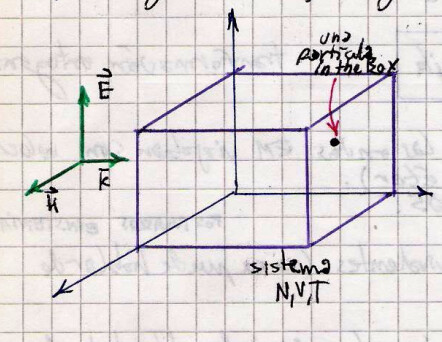
\includegraphics[width=0.35\textwidth]{images/fig_ft1_problema8.jpg} 
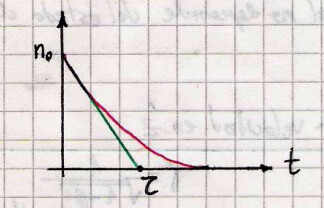
\includegraphics[width=0.35\textwidth]{images/fig_ft1_problema8B.jpg} 

Como el campo es armónico la velocidad $\vb{v}$ será armónica $ \vb{v} = \vb{v}_0 \euler^{- i \omega t} $,
donde $ \nu \equiv 1 / \tau $ es la frecuencia entre choques.
Simplificamos la exponencial temporal
\[
	i \omega m \vb{v}_0 = e \vb{E}_0 - \frac{m}{\tau} \vb{v}_0
\]
\[
	\vb{v}_0 = \frac{e\tau}{m} \frac{1}{1-i\omega\tau} \vb{E}_0.
\]
Entonces para la corriente en promedio tenemos
\[
	\vb{J} = n e \vb{v}_0 = \frac{n e^2 \tau}{m} \frac{1}{1-i\omega\tau} \vb{E}_0
\]
donde el factor del campo sub-cero puede verse como un $\sigma(\omega)$, y entonces
podemos escribir
\[
	\vb{J} = \frac{ \sigma(0) }{1 - i \omega \tau } \vb{E}_0
\]
donde si $\omega \tau \gg 1$ tiro el uno y tengo un desfasaje de 90$^\circ$ ($-i$).

La siguiente picture muestra diversos comportamientos en función de la frecuencia $\omega$.
Puntualmente con $\omega \gg \nu$ tenemos una frecuencia de choques muy baja (gas ionizado)
partículas muy alejadas entre sí.

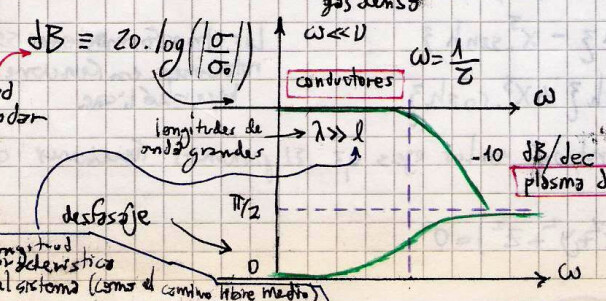
\includegraphics[width=0.5\textwidth]{images/fig_ft1_problema8C.jpg} 

Tenemos la siguiente observación que debería pasarse a texto o ilustrar de otra manera, o quiźas
mejor entender en qué sentido van las longitudes de onda (las ondas EM son transversales).

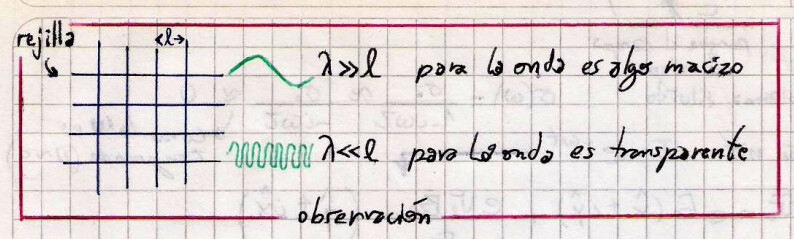
\includegraphics[width=0.35\textwidth]{images/fig_ft1_problema8F.jpg} 

Con toda esta información podemos resolver las ecuaciones de Maxwell faltantes.
Estamos con
\[
	\sigma(\omega) = \frac{i \sigma_0}{\omega \tau} = \frac{ i n e^2}{ m \omega }
\]
con $\omega \tau \gg 1$ y debemos resolver
\[
	\rotorm{E} = - \frac{1}{c} \dpar{\vb{B}}{t}
\]
\[
	\rotorm{H} = \frac{4\pi}{c}\vb{J} + \frac{1}{c} \dpar{\vb{E}}{t}
\]
Entonces tomo la primera y la introduzco en la segunda, luego
\[
	\Nabla\times\Nabla\times\vb{E} = - \frac{1}{c}\dpar{}{t}(\rotorm{B})
\]
que resulta en
\[
	\lapm{E} + K^2 E = 0,
\]
donde
\[
	K^2 = \Frac{\omega}{c}^2 \left[ 1 + \frac{i 4 \pi \sigma}{\omega}\right]
\]
de lo cual extraemos
\[
	\frac{k}{\omega} = \frac{1}{c} \sqrt{ 1 - \frac{4\pi n e^2}{m \omega^2} }
\]
y podemos definir una $\omega_P^2 \equiv 4\pi n e^2 / m$ que es una frecuencia del plasma típica.
Luego, si $k/\omega$ es un número real tenemos una onda que se propaga pues implica que
$\omega > \omega_P $ y $K$ es real entonces $E_0 \euler^{i (kx-\omega t)}$.
Por el contrario si $k/\omega$ es un número imaginario tenemos una onda que se atenúa y 
$ \omega < \omega_P $ y el $K$ es imaginario lo cual lleva a a $E_0 \euler^{-|k|x}\euler^{i i\omega t)}$,
que significa que la onda no puede penetrar el medio y empieza a decaer.

El típico modelo de un plasma es la ionosfera. Véase la siguiente nota:

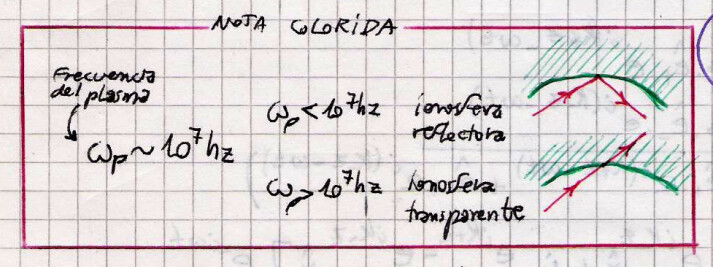
\includegraphics[width=0.45\textwidth]{images/fig_ft1_problema8D.jpg} 

La radio AM refleja y tiene más alcance. La radio FM en cambio deja pasar y se va al espacio.

{\bf Observación}

Esto que sigue parece ser un tema nuevo, así que no correspondería realmente a este ejemplo.
Tenemos un campo magnético fuerte.
Una onda $\vb{E}$ linealmente polarizada (se puede ver como superposición de dos polarizaciones
circulares)
\[
	\vb{E} = E_0 ( \xver \pm i \yver ) \euler^{i (kz -\omega t)}
\]

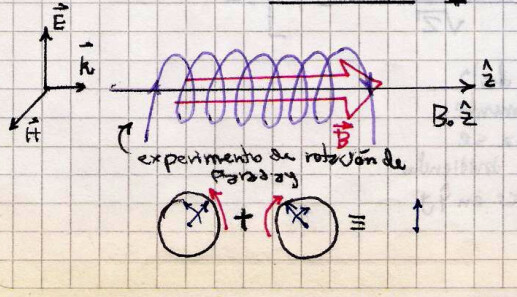
\includegraphics[width=0.35\textwidth]{images/fig_ft1_problema8E.jpg} 

Escribimos, sin incluir la fuerza viscosa, pero sí el campo magnético porque es intenso, luego
\[
	m \dtot{\vb{v}}{t} \approx e \vb{E} + e \left( \frac{\vb{v}}{c} \times B_0\zver \right)
\]
Trabajo en la zona de plasma diluído
\[
	\sigma(\omega) = \frac{\sigma_0}{1-i\omega\tau} \approx -\frac{\sigma_0}{i\omega\tau} \sim 0,
\]
donde lo último es porque la frecuencia es muy grande.
Usando la aproximación vista de que $ E \sim \euler^{ i \omega t } $
\[
	- i m \omega \vb{v}_0 = e E_0 (\xver \pm \yver ) + \frac{e v_0 B_0 }{c} (-\yver \pm i\xver ) 
\]
y tenemos el sistemita [?]
\[
	\begin{cases}
	- i m \omega v_0 = eE_0 \pm i \frac{e v_0 B_0}{c} \\
	\\
	\pm m \omega v_0 = \pm i e E_0 - \frac{e v_0 B_0}{c}
	\end{cases}
\]
de manera que
\[
	v_0 = \frac{ i e E_0}{m( \omega \pm e B_0 / (mc) )}
\]
luego, como $ J = n e v_0$ se tiene
\[
	J = \frac{ i n e^2 }{m( \omega \pm e B_0 / (mc) )} E_0
\]
donde 
\[
	\omega_c \equiv \frac{e B_0}{m c},
\]
es la llamada frecuencia de ciclotrón. Tenemos dos $\sigma$. Se sigue que
\[
	\frac{K}{\omega} = \frac{1}{c} \sqrt{ 1 - \frac{ \omega_P^2 }{ \omega (\omega \pm \omega_C )} }
\]
entonces la raíz en el rhs es una especie de índice de refracción $n_r = n\pm$.

Las dos ondas circularmente polarizadas ven diferentes índices de refracción.
Tomo
\[
	\frac{ \xver \pm i \yver }{\sqrt{2}} \equiv \hat{e}_{\pm}
\]
y, absorbiendo la $\sqrt{2}$ en la amplitud $E_0$ se tiene
\[
	\vb{E} = \vb{E}_+ + \vb{E}_- = 
	E_0 \: \left( \hat{e}_{+} \euler^{i (K_+z -\omega t)} +
	+ \hat{e}_{-} \euler^{i (K_-z -\omega t)} \right)
\]
\[
	\vb{E} = \vb{E}_+ + \vb{E}_- = 
	E_0 \: \left( \frac{ \euler^{i K_+ z } + \euler^{ i K_- z } }{\sqrt{2}}\xver +
	i \frac{ \euler^{i K_+ z} - \euler^{i K_- z }}{\sqrt{2}} \yver \right) 
	\euler^{ -i \omega t }
\]
El ángulo $\alpha$ de la onda linealmente polarizada se obtiene dividiendo las partes
en $\xver$ y en $\yver$.
Así tendremos
\[
	\tan\vp = \frac{\euler^{i K_+ z} - \euler^{i K_- z }}{\euler^{i K_+ z} + \euler^{i K_- z }}
\]
y esta expresión se puede ``simetrizar'' para obtener
\[
	\tan\vp = \frac{\euler^{i ( K_+/2 - K_-/2 ) z} - \euler^{- i ( K_+/2 - K_-/2 ) z }}
	{ \euler^{i  ( K_+/2 - K_-/2 )  z} + \euler^{-i ( K_+/2 - K_-/2 ) z } }
\]
\[
	\tan \vp = \tan\Frac{(K_+ - K_-)z}{2}
\]
y como $K_+ =\omega/c \: n_+$ y $K_- =\omega/c \: n_-$ se tiene finalmente
\[
	\vp = \frac{\omega z}{2c}( n_+ - n_- ).
\]
  
\end{ejemplo}

\begin{ejemplo}{\bf Problema 4. Mixed tips}

Tenemos un mal conductor (un conductor pobre) y un buen conductor.
La ecuación general es
\[
	\lapm{E} + \frac{\mu\varepsilon\omega^2}{c^2}
	\left[ 1 + i \frac{4\pi\sigma}{\omega\varepsilon}\right] E =0
\]
donde toda la constante que acompaña al campo es una $K^2$ efectiva (para que tengamos una
ecuación de Helmholtz). Luego en un conductor bueno desprecio el 1 porque $\sigma$ es
constante y muy grande. En un conductor magro no se puede despreciar el 1 claramente porque
$\sigma$ es muy pequeño y entonces tengo dos expresiones para $K^2$. En este último caso
aproximamos $ K = \sqrt{1 + \chi }\sim 1 + 1/2 \:\chi$.
Entonces
\[
	K \approx (1+i)\frac{\sqrt{2\pi\sigma\mu\omega}}{c} = \frac{1+i}{\delta} \qquad \qquad
	K \approx \sqrt{\mu\varepsilon} \frac{\omega}{c}\left[ 1 + i \frac{2\pi\sigma}{\omega\varepsilon}\right]
\]
para conductor bueno y magro, respectivamente.
El siguiente gráfico ilustra los diferentes comportamientos

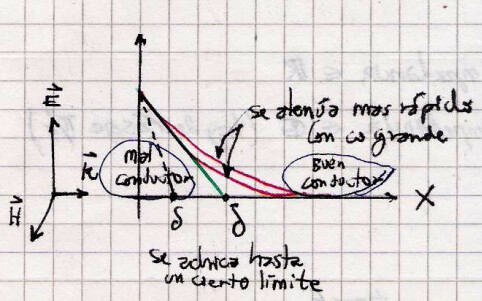
\includegraphics[width=0.40\textwidth]{images/fig_ft1_problema4A.jpg} 

En el problema se piden calcular
$ \vm{\mu_E}, \vm{\mu_H}, \vm{W} = \vm{\pe{J}{E}}$ siendo esta última la energía disipada
por efecto Joule.

Digamos en sumario que un buen conductor disipa más energía; $\mu_E$ disminuye y
$\mu_E < \mu_B$, es más magnético que eléctrico. Por lo tanto el material se comporta
de forma inductiva. Un conductor magro en cambio disipa menos energía, entonces
$\mu_E > \mu_B$, el conductor expulsa corriente y el material se comporta en forma
capacitiva.

Se define el factor de mérito $Q$ de la siguiente forma (una cuenta que haremos para un
buen y para un mal conductor)
\[
	Q \equiv \omega \frac{ \vm{\mu} }{ \vm{W}} =
	\begin{cases}
	\displaystyle \frac{\varepsilon \omega}{4 \pi \sigma} \gg 1 &\qquad \text{ mal conductor } \\
	\\
	\displaystyle \frac{1}{2} &\qquad \text{ buen conductor}
	\end{cases}
\]
Se ve que para el caso de buen conductor la relación entre la energía en el campo y la
disipada es fija y no depende de nada.

{\bf Otra cosa}

¿Pero qué sucede cuando una onda atraviesa un conductor bueno en el contorno?
La situación está depicted en el gráfico siguiente:

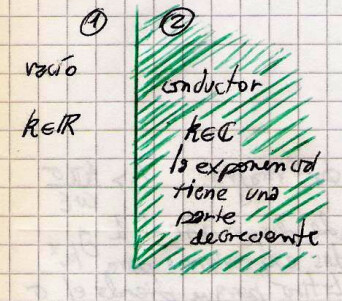
\includegraphics[width=0.40\textwidth]{images/fig_ft1_problema4B.jpg} 

\[
	\begin{cases}
	 E_{t_2} - E_{t_1} = 0 \\
	 \\
	 H_{t_2} - H_{t_1} = \frac{4 \pi}{c} g \quad \text{ perfecto }
	\end{cases}
\]
y vemos que no hay deltas en el rhs de la segunda condición [?]. En el caso de conductor bueno
(no perfecto) se tiene un cero y entonces $  H_{t_2} - H_{t_1} = 0 $.

En la zona $\textcircled{1}$
\[
	\vb{E}_1 = E_0 \: \euler^{i (K_1x - \omega t)} \yver  \qquad \qquad 
	\vb{H}_1 = \frac{c}{\mu \omega} \pv{k_1}{E_1} = \frac{E_0}{\sqrt{\mu/\varepsilon}} 
	\euler^{i (k_1x - \omega t)} \zver
\]

En la zona $\textcircled{2}$, teniendo en cuenta que aquí $k_2 = (1 + i) / \delta$ resulta
\[
	\vb{E}_2 = E_0 \euler^{-x/\delta} \euler^{i (x/\delta - \omega t)} \xver
	\qquad \qquad 
	\vb{H}_2 = \frac{E_0 \euler^{-x/\delta} \euler^{i (x/\delta - \omega t)} }
	{ \sqrt{\mu/\varepsilon} \sqrt{\omega\varepsilon/(4\pi\sigma)} \euler{-i\pi/4} }\xver
\]
\notamargen{Check que el campo $\vb{H}$ sea en $x$ versor.}

Y vemos que $\vb{H}$ siempre se puede llevar al campo $\vb{E}$ sobre algo que tiene unidades
de impedancia.
En la zona $\textcircled{1}$ los campos $\vb{E}, \vb{B}$ viajan en fase pues la impedancia es un
número real. En la zona $\textcircled{2}$ los campos viajan desfasados porque la impedancia es
compleja; hay un desfasaje de $\pi/4$.
 
\end{ejemplo}

\begin{ejemplo}{\bf Problema 7 (Experiencia de Wiener)}

Se muestra en la figuretta un conductor perfecto, un espejo perfecto.

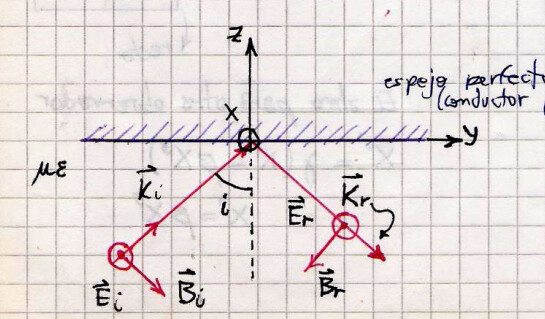
\includegraphics[width=0.40\textwidth]{images/fig_ft1_problema7A_ondas.jpg} 

Planteamos las prescripciones de los campos, dado el sistema coordenado.
\[
	\vb{B} = \sqrt{\mu\vare} \:\pv{k}{E}
\]
\[
	\vb{E}_i = E_i \euler^{ i ( \pe{k_i}{x} - \omega t )} \xver \qquad \qquad 
	\vb{B}_i = \sqrt{\mu\vare} \: E_i \: \euler^{ i ( \pe{k_i}{x} - \omega t ) } 
	\hat{k}_i\times\hat{x}
\]
\[
	\vb{E}_r = E_r \euler^{ i ( \pe{k_r}{x} - \omega t )} \xver \qquad \qquad 
	\vb{B}_r = \sqrt{\mu\vare} \: E_r \: \euler^{ i ( \pe{k_r}{x} - \omega t ) } 
	\hat{k}_r\times\hat{x}
\]

Evaluaremos los contornos. En el material el campo eléctrico es nulo, pero el contorno
asociado al campo magnético no es nulo porque hay densidad de corriente superficial al
rebotar la onda incidente,
\[
	E_r + E_i = 0 \qquad \qquad ( \vb{B}_i + \vb{B}_r ) \times \hat{n} = 0
\]
\notamargen{El producto escalar $ ( \vb{B}_i + \vb{B}_r ) \cdot \hat{n} $ lleva en
realidad a la ley de Snell.}
Podemos descomponer los vectores de onda según
\[
	\vb{k}_i = \vb{k}_y + \vb{k}_z \qquad \qquad 
	\vb{k}_r = \vb{k}_y - \vb{k}_z 
\]
donde 
\[
	k_y = |k|\sin( i) \qquad k_z = |k|\cos( i) .
\]
Entonces
\[
	\vb{E} = E_i ( \euler^{ i ( \pe{k_i}{x} - \omega t)} - 
	\euler^{i ( \pe{k_r}{x} - \omega t)} ) \xver
\]
y los vectoriales son
\[
	\hat{k}_i \times \xver = - \sin(i) \zver + \cos(i) \yver
	\qquad \qquad 
	\hat{k}_r \times \xver = - \sin(i) \zver - \cos(i) \yver
\]
de manera que el campo magnético
\[
	\vb{B} = -E_i \sqrt{\mu\vare} 
	\left[ 
	( \euler^{ i ( \pe{k_i}{x} - \omega t)} - \euler^{i ( \pe{k_r}{x} - \omega t)} ) 
	\sin(i) \zver
	( \euler^{ i ( \pe{k_i}{x} - \omega t)} + \euler^{i ( \pe{k_r}{x} - \omega t)} ) 
	\cos(i) \yver
	\right]
\]

Simplificando un poco las expresiones anteriores,
\[
	\vb{E} = 2 i E_i \euler^{ i k_i y } \euler^{ - i \omega t)} \sin( k_z z )
\]
\[
	\vb{B} = 2 E_i \sqrt{\mu\vare} \euler^{ i k_i y } 
	\left[ 
	- i \sin( k_z z ) \sin(i ) \zver +
	\cos( k_z z ) \cos(i ) \yver
	\right]
\]
y entonces el vector de Poynting 
\[
	\vm{\vb{S}} = \frac{c}{8\pi \mu} \mathcal{Re}( \vb{E}^* \times \vb{B} )
\]
resulta
\[
	\vm{\vb{S}} = \frac{c}{8\pi \mu} 4 \sqrt{\mu\vare} E_i^2 \sin^2(k_z z )\sin(i) \yver,
\]
tenemos flujo en la dirección $\yver$. Se tienen, además,
\[
	\vm{\mu_E} = \frac{\vare}{16\pi} 4 E_i^2 \sin^(k_z z) 
\]
\[
	\vm{\mu_M} = \frac{\vare}{4\pi} E_i^2 
	\left(
	\sin^2(k_zz) \sin^2(i) + \cos^2(k_zz) \cos^2(i)
	\right)
\]
Con incidencia normal $i=0$ se tiene vector de Poynting promedio nulo. Hay ondas estacionarias
en ese caso.

{\bf Incidencia normal}

Consideramos $i=0$ ahora. El Poynting promedio es nulo, pero 
\[
	\vm{\mu_E} = \frac{\vare}{4\pi} E_i^2 \sin^(k_z z) 
	\qquad 
	\vm{\mu_M} = \frac{\vare}{4\pi} E_i^2 \cos^2(k_zz) \cos^2(i) 
\]

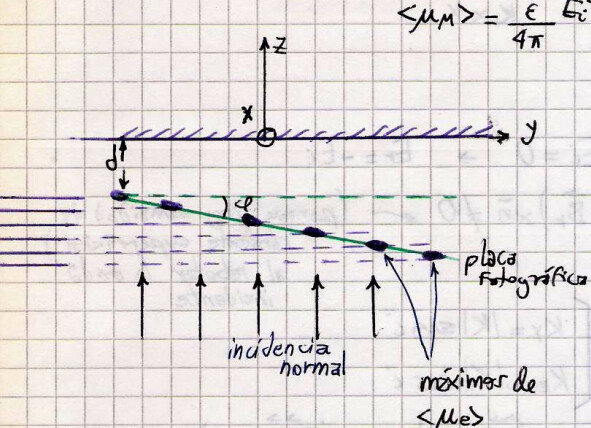
\includegraphics[width=0.40\textwidth]{images/fig_ft1_problema7B_ondas.jpg} 

En $ z = 0 $ se tienen $ \vm{\mu_E} = 0 $ y $ \vm{\mu_M} \neq 0$ si la placa está en $\vp=0, z=0$
no se registra nada y entonces $\vb{E}$ es el vector óptico.

Cuando $ \vp \neq 0 $ y existe un $ d > 0 $  se imprimen franjas oscuras en los máximos de $E$.
El máximo de $ \vm{\mu_E} $ vendrá de la cuenta
\[
	kz = \left( n + \frac{1}{2}\right) \pi
\]
y será 
\[
	z_M = \frac{\lambda}{2} \left( n + \frac{1}{2}\right)
\]
con un espaciamiento entre máximos (interfranja) de $ \Delta D = 1 / (2\sin\vp)$.

{\bf Incidencia 45$^\circ$}

La incidencia es $ i = \pi / 4 $ y entonces seno y coseno dan lo mismo $1/\sqrt{2}$ de modo
que el TE nos da la información
\[
	\vm{\mu_E} = \frac{\vare}{16\pi} 4 E_i^2 \sin^(k_z z / \sqrt{2})  \qquad 
	z_M = \frac{\lambda}{\sqrt{2}} \left( n + \frac{1}{2}\right) \qquad 
	\Delta D = \frac{ 1 }{ ( \sqrt{2} \sin\vp ) }
\]

Para el TM no hace falta hacer las cuentas nuevamente. Es similar al TE pero con $\vb{E}=\vb{B}$
de manera que $ \vm{\mu_E}^{\text{TM}} = \vm{\mu_B}^{\text{TE}} $ y será
\[
	\vm{\mu_B}^{\text{TE}} = \frac{\vare}{8\pi} E_i^2,
\]
que es uniforme (no hay franjas).
 
\end{ejemplo}

\begin{ejemplo}{\bf Problema 5 (presión de radiación)}

Veamos el dibujete

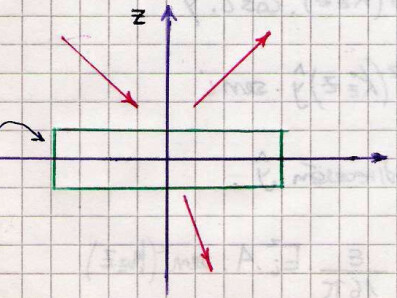
\includegraphics[width=0.40\textwidth]{images/fig_ft1_problema5_ondas.jpg}

No me interesará la componente tangencial porque se hace tender la pared a cero.
Se evaluarán
\[
	\int_S T\nver dS - \int_V \dpar{\vb{g}}{t} dV.
\]
donde $\vb{g}$ es la densidad de momento lineal del campo electromagnético.
 
\end{ejemplo}



% \bibliographystyle{CBFT-apa-good}	% (uses file "apa-good.bst")
% \bibliography{CBFT.Referencias} % La base de datos bibliográfica

\end{document} 
